Our goal in this work is to \emph{test what is being executed}. To achieve this we developed a new software engineering methodology for testing distributed systems, implemented on top of the \psharp framework. The original \psharp framework is explain in Section~\ref{sec:overview:psharp}, while the new approach is explained in Section~\ref{}.

\subsection{The \psharp framework}
\label{sec:method:psharp}

\psharp~\cite{deligiannis2015psharp} provides an \emph{event-driven asynchronous programming} language and a \emph{systematic concurrency testing} engine for developing highly-reliable distributed systems.

The \psharp language is an extension of \csharp, built on top of Microsoft's Roslyn\footnote{\url{https://github.com/dotnet/roslyn}} compiler, that enables asynchronous programming using communicating state-machines. \psharp machines can interact asynchronously by sending and receiving events,\footnote{We use the word ``event'' and ``message'' interchangeably.} an approach commonly used to develop distributed systems. This programming model is similar to actor-based approaches provided by other asynchronous programming languages (e.g. Scala~\cite{odersky2008programming} and Erlang~\cite{armstrong1996erlang}).

A \psharp machine consists of an input event queue, states, state transitions, event handlers, fields and methods. Machines run concurrently with each other, each executing an event handling loop that dequeues an event from the input queue and handles it by invoking an appropriate event handler. This handler might update a field, create a new machine, or send an event to another machine. In \psharp, a send operation is non-blocking; the message is simply enqueued into the input queue of the target machine, and it is up to the operating system scheduler to decide when to dequeue an event and handle it. All this functionality is provided in a lightweight runtime library, build on top of Microsoft's Task Parallel Library~\cite{leijen2009tpl}.

Because \psharp is built on top of \csharp, the programmer can blend \psharp and \csharp code; this not only lowers the overhead of learning a new language, but also allows \psharp to easily integrate with legacy code. Another advantage is that the programmer can use the familiar programming and debugging environment of Visual Studio.

A key capability of the \psharp runtime is that it can run in \emph{bug-finding mode}, where a embedded systematic testing engine captures and takes control of all sources of nondeterminism (such as event handler interleavings, failures, and client requests) in a \psharp program, and then systematically explores all possible executions to discover bugs.

\psharp is available as open-source\footnote{\url{https://github.com/p-org/PSharp}} and is currently used by various teams in Microsoft to develop and test distributed protocols and systems.

\PDComment{Do we want to actually mention (and compare with) P in this paper?}
%The \psharp language belongs to the same family of languages as P~\cite{desai2013p}.

\subsection{Methodology}
\label{sec:method:new}

In previous work~\cite{deligiannis2015psharp}, we approached the problem of testing legacy distributed systems as follows. First, we ported the system to \psharp, then we modeled its environment as \psharp state machines, and finally we tested the ported system and its environmental model using the \psharp systematic concurrency testing engine. The limitation of this approach is that it does not allow us to directly test a legacy system, as it has to be re-implemented first in \psharp. However, such endeavor is very costly and time consuming, and thus is not realistic for testing an existing production system, such as the Azure Storage vNext. Also, unless the code under test is the one that will actually execute, there is no guarantee that the real system will be bug-free.

In order to solve this problem, and allow \psharp to be used for testing legacy distributed systems, we decided to take a radically different modeling approach. We provide the capability to model the environment of a system using \psharp, and then allow the developer to take advantage of existing language features, such as \emph{method dispatch}, to connect the system under test with the environmental model, and finally test it using the \psharp systematic concurrency testing engine.

We argue that our approach is \emph{flexible} since it allows the user to model \emph{as much} or \emph{as little} of the environment as required to achieve the desired level of testing. We also argue that our approach is \emph{generic} since a programmer can build on top of it to test more complicated use cases (see Section~\ref{}). Furthermore, the language features that are required to be used to connect the real code with the modeled code, are already being heavily used in production for testing purposes, which makes this method approachable to product groups.

\begin{figure}[t]
\centering
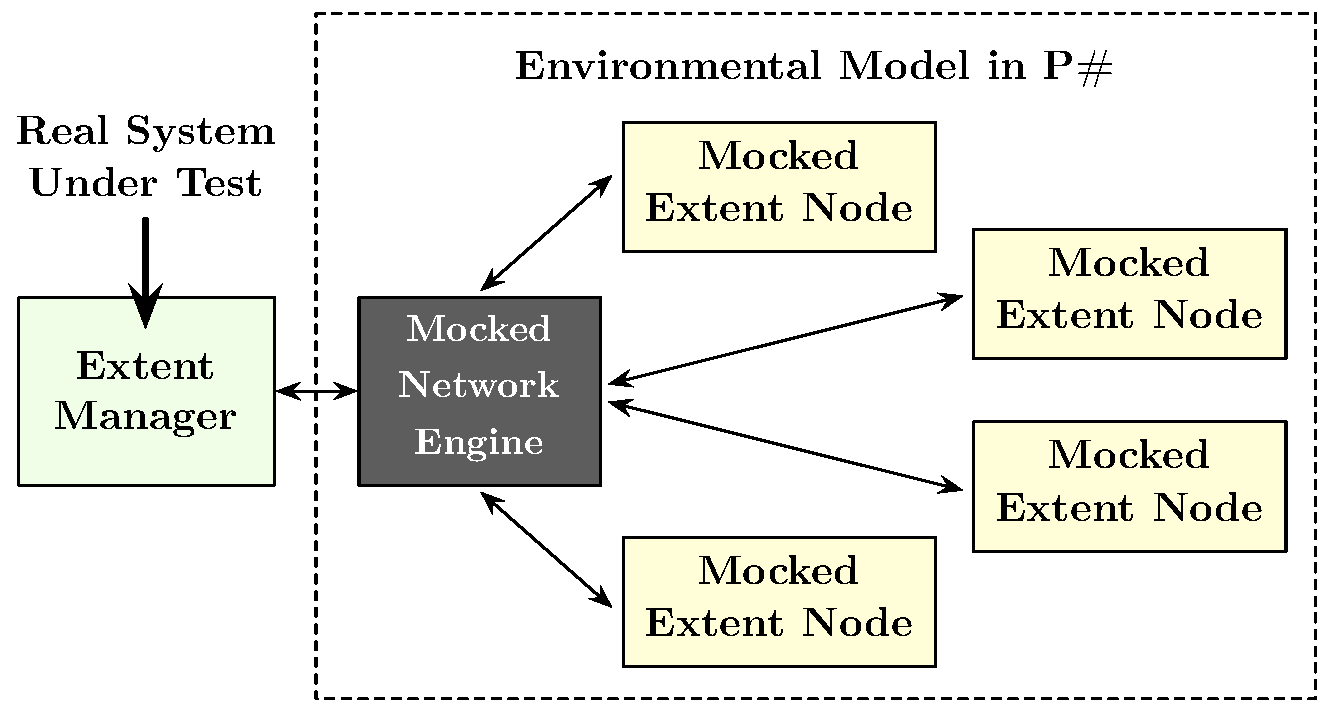
\includegraphics[width=\linewidth]{img/mocked_engine}
\caption{The real environment of the Extent Manager is replaced with a mocked version for testing.}
\label{fig:azurestoremodel}
\end{figure}

\subsection{Modeling the environment}
\label{sec:method:model}

Draft.

\subsection{Using method dispatch for modeling}
\label{sec:method:dd}

Method dispatch is the process of selecting which method, from a set of available methods with the same interface, should be invoked during a program's execution. There are two types of method dispatch: \emph{static}, which is resolved during compilation; and \emph{dynamic}, which is resolved in runtime.  \csharp (and thus \psharp) supports both static and dynamic dispatch, and provide the \texttt{virtual} modifier that can be used to declare a method which can be \emph{overridden} during runtime by an inheriting class. This capability is provided by the common language runtime (CLR) of Microsoft's .NET framework, and is a key feature of \csharp as well as other mainstream object-oriented languages.

Using method dispatch for modeling is straightforward. The system under test exposes a set of APIs as \emph{virtual methods}. The developer can then \emph{override} these APIs and replace them with \emph{mocks} that will execute instead of the original implementations during systematic testing with \psharp.

We now give an example of using dynamic dispatch to model the network engine of an extent manager in the Azure Storage vNext case study (see Figure~\ref{fig:enginecode}). The network engine is responsible for sending to and receiving messages from the various components of the system. During real execution, the network engine uses a custom remote procedure call (RPC) .NET library for communication. For testing, though, it is desirable to replace all calls to this RPC library with \psharp send and receive operations, which can be captured and systematically interleaved to find bugs. We easily achieved this by exposing the original send message operation of the network engine as a virtual method, and then overriding it for testing. In the overridden method, we created a \psharp event and then we wrapped the original message in this event's payload. Then, instead of invoking the RPC library, we invoke the \texttt{PSharpRuntime.Send(...)} method, which asynchronously sends the event (containing the original message) to the target extent node machine.

For mocking the receive operation, we take advantage of the implicit receive of events in \psharp machines. When a extent node machine receives an event, an appropriate event handler is invoked, which extracts the original message from the payload and then handles it accordingly.

\begin{figure}[t]
\begin{lstlisting}
// Public interface of the real network engine
class NetworkEngine {
  public virtual void SendMessage();
  public virtual void EnqueueMessage();
}

// The mocked network engine used during testing
class MockedNetEngine : NetworkEngine {
  ExtentManager EM; // Handle to actual system under test
  MachineId Env; // Handle to modeled environment
  
  public MockedNetEngine(ExtentManager em, MachineId env) {
    this.EM = em;
    this.Env = env;
  }
  
  public override void SendMessage(Socket s, Message msg) {
    PSharpRuntime.Send(this.Env, new MsgEvent(), s, msg);
  }
  
  public override void EnqueueMessage(Message msg) {
    this.EM.ProcessMessage(msg);
  }
}
\end{lstlisting}
\vspace{-2mm}
\caption{The mocked network engine used for testing the Azure Storage vNext system.}
\label{fig:enginecode}
%\vspace{-2mm}
\end{figure}

Another important operation that we had to model in order to capture the nondeterminism in  the Azure Storage vNext system, and be able to detect the liveness violation, was to model the timer operation that sends a heartbeat every 5 seconds and a sync message every 5 minutes.

\subsection{Extensibility of the \psharp framework}
\label{sec:method:extend}

Async/Await

custom schedulers, etc

Logs/traces -> user can extend them?

\PDComment{mention dependency injection pattern?}
